\documentclass[pdftex,12pt,oneside,a4paper,spanish, english, brazil]{abntex2}
\PassOptionsToPackage{english}{babel}

% ----------------------------------------------------------------------------------------
% - PACOTES
  \usepackage{sty/configs}                  % Pacotes utilizados
  \usepackage{sty/metadados_rt}             % Dados do órgão / cliente
  \usepackage{sty/dados_cpai}               % Dados do CPAI/FUB
  \usepackage{sty/vocabulario}              % Vocabulário específico do projeto
  \usepackage{sty/leiaute_rt}               % Definições de layout do documento

% ----------------------------------------------------------------------------------------
\addto\captionsbrazil{
	%% ajusta nomes padroes do babel
	\renewcommand{\bibname}{Indice}
	\renewcommand{\contentsname}{Indice}
	\renewcommand{\indexname}{\’Indice}
	\renewcommand{\listfigurename}{Lista de ilustra\c{c}\~{o}es}
	\renewcommand{\listtablename}{Lista de tabelas}
	%% ajusta nomes usados com a macro \autoref
	\renewcommand{\pageautorefname}{p\’agina}
	\renewcommand{\sectionautorefname}{se{\c c}\~ao}
	\renewcommand{\subsectionautorefname}{subse{\c c}\~ao}
	\renewcommand{\paragraphautorefname}{par\’agrafo}
	\renewcommand{\subsubsectionautorefname}{subse{\c c}\~ao}
}

% ----------------------------------------------------------------------------------------
% - INÍCIO DO DOCUMENTO
  \begin{document}
      \begin{sloppypar}
          
          % Seleciona o idioma do documento (conforme pacotes do babel)
            %\selectlanguage{english}
            %\selectlanguage{spanish}
            
          % Retira espaço extra obsoleto entre as frases.
            \frenchspacing
          
          % ------------------------------------------------------------------------------
          % - ESTRUTURA DO DOCUMENTO
          % ------------------------------------------------------------------------------
          % ------------------------------------------------------------------------------
          % - PRÉ-TEXTUAL
          % ------------------------------------------------------------------------------
          \pretextual

          % Capa
            %~~~~~~~~~~~~~~~~~~~~~~~~~~~~~~~~~~~~~~~~~~~~~~~~~~~~~~~~~~~~~~~~~~~~~
% File  : capa
%~~~~~~~~~~~~~~~~~~~~~~~~~~~~~~~~~~~~~~~~~~~~~~~~~~~~~~~~~~~~~~~~~~~~~

% Limpa os estilos de página
  \thispagestyle{empty}

% Desenho no fundo da página
  \ThisCenterWallPaper{1}{img/CapaTR3.pdf}

% Cria uma mini-página para inserir os dados da capa usando 70% da largura do texto
  \begin{flushright}

    \begin{minipage}{0.6\textwidth}
      \begin{flushleft}
          \sffamily
          % Parte superior da capa
          \vspace{2cm}
          \LARGE \textbf{Requerimientos de Alcance PV, FV} \\
          \footnotesize \textcolor{black!60}{\rtid} \\[1cm]
          \Huge \textbf{\rttitulo} \\
      \end{flushleft}
    \end{minipage}%

    \vfill
    \begin{minipage}{0.6\textwidth}
        \begin{center}
          % Rodapé da capa
          \sffamily
          \small \rtlocal \\
          Versión \rtversao \\
          \rtdata \\
        \end{center}
    \end{minipage}%
  \end{flushright}

            \cleardoublepage
          

          % Filiação CPAI
            %%~~~~~~~~~~~~~~~~~~~~~~~~~~~~~~~~~~~~~~~~~~~~~~~~~~~~~~~~~~~~~~~~~~~~~
% File  : filiacao_cpai
%~~~~~~~~~~~~~~~~~~~~~~~~~~~~~~~~~~~~~~~~~~~~~~~~~~~~~~~~~~~~~~~~~~~~~

%---------------------------------------------------------------------
{
\ABNTEXchapterfont\setlength{\parindent}{0cm}
\textsf{\textbf{New Digital Partnerts} }

{\scriptsize \textsf{\textbf{Gerencia de Desarrollo}}} \\ 
\textsc{Nombre}


%---------------------------------------------------------------------
\vspace{0.8cm}

\vfill
\textsf{\textbf{Cargo}} \\
\textsc{Nombre} \\

\textsf{\textbf{Equipo de Desarrollo}}

%\textsc{Ângelo Henrique Gonçalves Ramim} {\scriptsize (Analista de Tecnologia)} \\
\textsc{Nombre1} \\
\textsc{Nombre1} \\
\textsc{Nombre1} \\
\textsc{Nombre1} \\
\textsc{Nombre1} \\
%---------------------------------------------------------------------
% Fim de arquivo
%~~~~~~~~~~~~~~~~~~~~~~~~~~~~~~~~~~~~~~~~~~~~~~~~~~~~~~~~~~~~~~~~~~~~~

            %\cleardoublepage

          % Inserir a ficha bibliografica
            %%~~~~~~~~~~~~~~~~~~~~~~~~~~~~~~~~~~~~~~~~~~~~~~~~~~~~~~~~~~~~~~~~~~~~~
%    File      : ficha_catalografica
%    Type      : TeX
%    Date      : Time-stamp: <Sunday,10 Novem 2013,18:59:18>
%
%    Content   : 
%~~~~~~~~~~~~~~~~~~~~~~~~~~~~~~~~~~~~~~~~~~~~~~~~~~~~~~~~~~~~~~~~~~~~~

%----------------------------------------------------------------------
% Ficha bibliografica
%----------------------------------------------------------------------

{
\ABNTEXchapterfont\setlength{\parindent}{0cm}

\vspace*{\fill} 

{\tiny \copyright\ \textit{copyright} \the\year\ CPAI -- Todos os direitos reservados}

%\imprimircassificacaoseguranca         % Não implementado nesta versão do modelo de RT

\vspace*{\fill} % Posição vertical

\begin{fichacatalografica}\ABNTEXchapterfont
    \vspace*{\fill} % Posição vertical
    \hrule % Linha horizontal
    \begin{center} % Minipage Centralizado
        \begin{minipage}[c]{13cm} % Largura
            \hspace{0.5cm} \rttitulo\ / \rtautor. --
            \imprimirlocal : Universidade de Brasília, \rtdata-
            
            \hspace{0.5cm} \pageref{LastPage} p. : il. (algumas color.) ; 29,7 cm.\\
            
            \hspace{0.5cm}
            \parbox[t]{\textwidth}{\rttipo~--~\CPAI, \rtdata.}
            
            \hspace{0.5cm}
            \parbox[t]{\textwidth}{Versão final.}\\
            
            \hspace{0.5cm}
            \parbox[t]{\textwidth}{ISSN: \rtissn}\\
            
            \hspace{0.5cm}
            1. \rtkeyworda
            2. \rtkeywordb
            %3. \rtkeywordc
            I. Título

            \begin{flushright}
                 CDD \rtcdd
            \end{flushright}
        \end{minipage}
    \end{center}
    \hrule
\end{fichacatalografica}

\cleardoublepage
}

%----------------------------------------------------------------------

          % Sumarios
            \vspace{1cm}
            %\tableofcontents
           
          % ------------------------------------------------------------------------------
          % - TEXTUAL
          % ------------------------------------------------------------------------------
          \textual
          
          
          % Capítulo
            \chapter{Configuracion}
            La solución de Punto de Venta tiene como objetivo proporcionar a las empresas una aplicación Web, a través de la cual sus respectivas tiendas puedan ofrecer y vender sus productos bajo el esquema retail.
            Asimismo, el POS se integra con diversos ERPs o sistemas legacy, actualmente el sistema se encuentra certificado para SAP Business One.
            
            
            \section{Actores}
            
            Que usuarios tendrían acceso al sistema?\\
            La Arquitectura sera parte de la propuesta de acuerdo a los requerimientos del cliente
            
            \begin{itemize}
            	\item USER(1): Administrador- Almacenero - Venta - Caja - Despacho. *Denominado "Supervisor Zonal"
            	\item USER(2): Almacenero - Venta - Caja - Despacho.
            \end{itemize}
            
            	    Observaciones *** no todas las tiendas tienen administrador, el administrador puede ser el único actor en una tienda\\
            	Solicitan tener la administración total de los Roles y editar los permisos de sus usuarios.

            \section{Arquitectura}
            Que tienen implementado actualmente para la solución?\\
            La Arquitectura forma se presentara como propuesta de acuerdo a los requerimientos del cliente.
            \section{Estructura de Tiendas}
            Cuantas tiendas tenemos, se esperan más?\\
            Cual es la configuración de actores en cada tienda?\\
            Cuales son sus Fechas y Horas pico?\\
            	Actualmente la afluencia en Tacna es del 80\%  con un promedio de 30 Facturas al día.\\
            	Tiendas:\\
            \begin{enumerate}
            	\item Moquegua: un USER(1) y un USER(2) 10 \% 
            	\item Hilo: un USER(2) 10 \%;
            	\item Tacna - ZoFra:  un USER(1) 80\%;
            	\item Tacna - San Martin: dos USER(2);
            	\item Tacna - Parque Industrial: dos USER(2);
            	\item Tacna - Viñari: dos USER(2);
            \end{enumerate}
            
            \chapter{Módulos Punto de Venta}
           	Agruparemos los Módulos del POS en Transacciones, Almacenamiento, Ventas y Widgets.
           	     \begin{figure}[h!]
           		\centering
           		\caption{PUNTO DE VENTAS} \label{fig:maia}
           		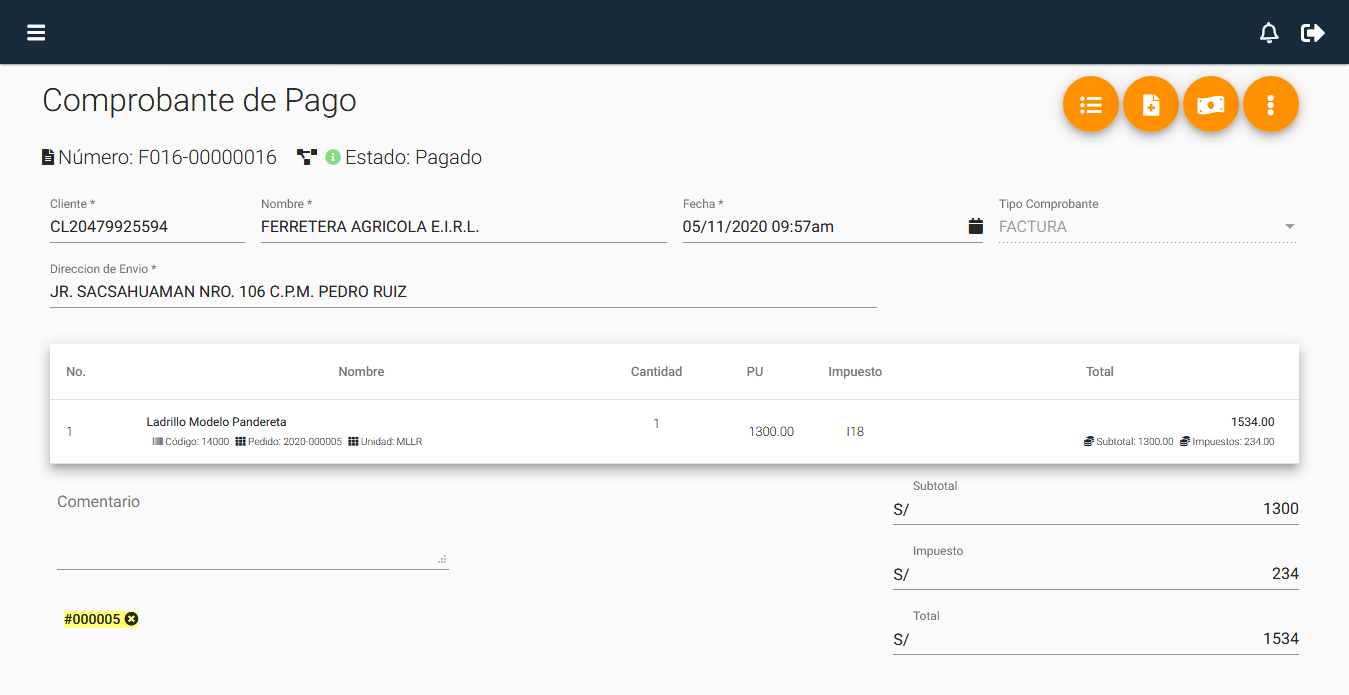
\includegraphics[width=0.6\linewidth,frame=0.5pt 5pt]{img/PV}
           	\end{figure}
              \section{Ventas}
              Gestiona todo el proceso de venta desde la cotización hasta colocar la orden de venta.
              \subsection{Orden de Venta}
             La orden de venta es un documento interno con la cual podremos iniciar el proceso de venta hacia nuestros clientes, en ella podremos definir información importante para su posterior facturación.\\
             Podemos encontrar en ella Widgets que dan soporte al vendedor para concretar sus ventas, que son: Muestras, Retornos, Resumen de Documentos, Confirmación de Picking, Clientes; para crear una orden de Venta consideraos el siguiente estándar:
             \begin{itemize}
              \item Elegir un cliente: se pueden elegir haciendo la búsqueda escribiendo directamente en la linea del cliente características como No de Documento (RUC, DNI) o partes del nombre o a través de un widget de búsqueda haciendo click en el icono de lupa; ademas de tener una lista de precio preferente la venta se realizara con la lista de precio del cliente elegido.\\
             Adicionalmente al hacer ENTER sobre la linea de cliente
             se añadira el "CLIENTE VARIOS".
             \item Selección de Productos: al clickear cada linea podemos acceder a una consola de búsqueda de artículos en la cual podremos buscar por SKU, Código de Barras y Parte del Nombre, luego de elegir el producto de linea podremos elegir la cantidad y unidad de medida (toma la primera), tenemos integrada un lector de Código de Barras Genérico para la búsqueda de productos.
             \item Cálculos: Los calculos son automáticos al interactuar con cada linea del se actualizan los datos de la misma y los calculos de cabecera.
             \end{itemize}
              Para continuar con el proceso de venta podremos poner la Orden de Venta en los estados de:
              \begin{itemize}
              	\item Enviado a Picking: esta función envía una alerta hacia almacén para un proceso de atención que finaliza enviando los productos a Despacho.
              	\item Guardado: podremos almacenar la OV a la espera de continuar con ella en un segundo momento.
              \end{itemize}
              Observaciones:
              \begin{itemize}
              	\item Las ventas al crédito están sujetas a supervisor o aprobación digital.
              	\item Esta venta Solo se crea en oficina Central.
              	\item Solo se crea a titulo gratuito solo se hace en Oficina Central no iría por PV.
              \end{itemize}
              \subsection{Venta Rápida}
              \begin{figure}[h!]
              	\centering
              	\caption{Ventas} \label{fig:maia}
              	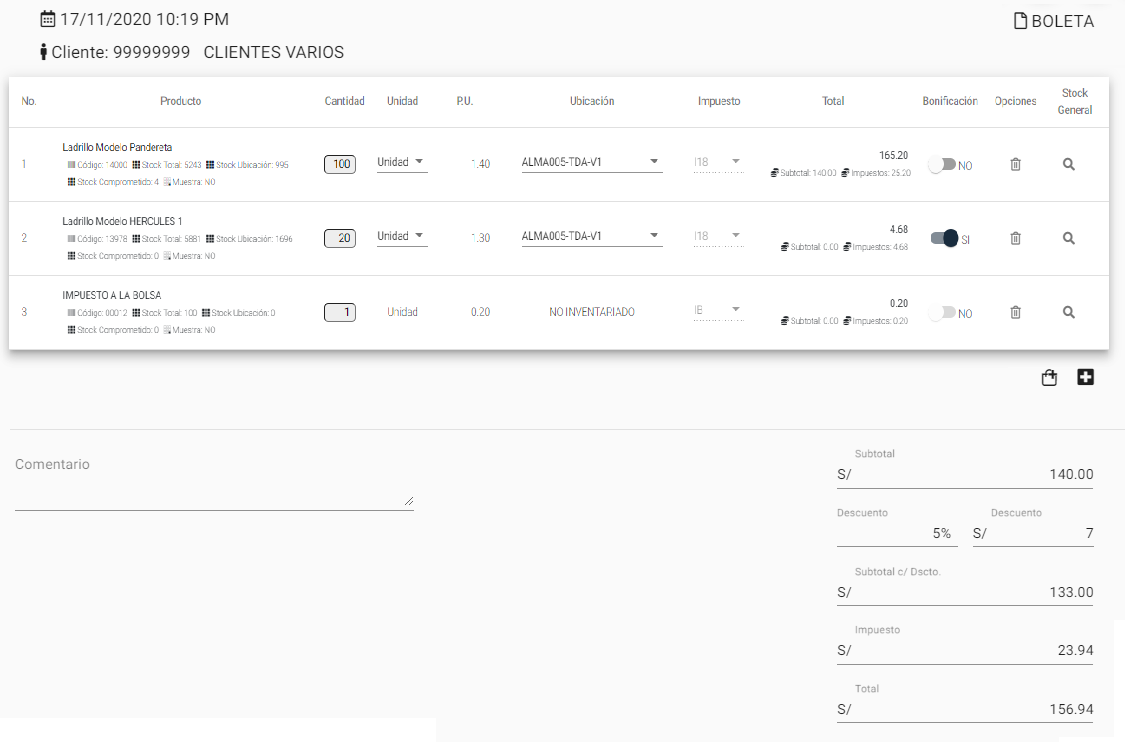
\includegraphics[width=0.65\linewidth,frame=0.5pt 5pt]{img/VENTA}
              \end{figure}
              La venta rápida tiene como finalidad generar todos los documentos asociados a una venta de manera que permita realizar el proceso completo de la venta; generando Orden de Venta, Movimiento de Existencias, Orden despacho, Comprobante desde una sola interfaz gráfica.\\
              
              El modulo cuenta con la integración de los maestros de productos, Lista de Precios y Almacenes, el proceso que se sigue para la venta rápida es el siguiente:
              \begin{itemize}
              	\item Elegir un cliente: se pueden elegir haciendo la búsqueda escribiendo directamente en la linea del cliente características como No de Documento (RUC, DNI) o partes del nombre o a través de un widget de búsqueda haciendo click en el icono de lupa; ademas de tener una lista de precio preferente la venta se realizara con la lista de precio del cliente elegido.\\
              	Adicionalmente al hacer ENTER sobre la linea de cliente
              	se añadira el "CLIENTE VARIOS".
              	\item Selección de Productos: al clickear cada linea podemos acceder a una consola de búsqueda de artículos en la cual podremos buscar por SKU, Código de Barras y Parte del Nombre, luego de elegir el producto de linea podremos elegir la cantidad y unidad de medida (toma la primera), tenemos integrada un lector de Código de Barras Genérico para la búsqueda de productos.
              	\item Cálculos: Los calculos son automáticos al interactuar con cada linea del se actualizan los datos de la misma y los calculos de cabecera.
              	\item *(1)Bonificaciones: Cada linea tiene un switch de ser una bonificación con lo cual el subtotal sera igual a 00.00, siento los impuestos igual al total de la linea.
              	\item *(2)Descuentos por Linea: En cada linea podremos incluir descuentos por importe o desuentos por porcentaje los cuales interactuan se actualizan entre si y se aplican al subtotal, con lo cual los impuestos se aplicaran sobre el "Subtotal con Descuento".
              	\item *(2)Opción de Transporte: El botón de transporte tiene pre-cargado una linea con Código de Producto, Precio Unitario Variable, Porcentaje de Detraccion y Código de detracción; activando la alerta de "Documento Afecto a Detracción a la espera de los requisitos mínimos para la afectación.
              	\item *(1)Opción de Bolsas: Se debe precisar que se ademas de aplicar los impuestos de afectación sobre este producto, la ley establece adicionalmente establece un IB(Impuesto a la bolsa); para lo cual tendremos un combo de bolsas con un botón que agrega al detalle una linea por el producto y
              	una linea  por el IB, de obsequiar la bolsa solo tendremos un botón que agrega el impuesto
              	por cada bolsa.
              	\item *(2)Descuentos en Cabecera: Se pueden aplicar descuentos al subtotal del documento por un importe o por un porcentaje aplicando los impuestos al "SubTotal con Descuento".
              \end{itemize}
          		(*)Funciones Opcionales, (1)Funciones Desarrolladas, (2)Funciones en Desarrollo; Se tiene el acceso al Widget de Clientes (Registro y Edición).
              \subsection{Cotización}
              Permite registrar una cotización de varios productos; asimismo se puede imprimir para entregársela al cliente.\\
              Observaciones:
              
              \begin{itemize}
                \item  Las cotizaciones registradas pueden convertirse posteriormente en órdenes de venta. 
                \item Se podrá enviar por correo.
                \item Las cotizaciones Se crearan en SAP y podrán ser transformadas a ventas desde el punto de venta.
                \item Se realizan regularmente en la tienda central.
                \item Las cotizaciones en el Punto de Venta son edita-bles de acuerdo a los factores del día actual.
              \end{itemize}
            \section{Almacenamiento}
            Estos módulos gestionan las alertas hacia almacén para gestionar la salida de los pedidos.
              \subsection{Movimiento de Existencias}
              Permiten mover de lógicamente los productos dentro de la tienda sin la necesidad de un documento adicional.\\
              Observaciones:
              \begin{itemize}
                \item Los movimientos serian virtuales para el cambio de ubicación de ventas a una ubicación de despacho.
                \item La transferencia entre tiendas son de caso muy particulares.
                \item Podría ser transferido a una ubicación de merma para ser trasladado posteriormente a otra tienda.
                \item Las transferencias de Items entre tiendas no están contemplados en el Punto de venta.
              \end{itemize}
              \subsection{Almacén - Despacho *No va por punto de Venta}
              En estos módulos se gestionan los movimientos de existencias como Alertas ordenadas de forma que se atiendas en el orden de tiempo previsto.
              Observaciones:
              \begin{itemize}
              	\item Se utilizara para finalizar las compras que están sujetas a aprobación.
              	\item También se utilizara para finalizar el proceso de facturas de reserva.
              \end{itemize}
              \subsection{Devoluciones}
              Este modulo permite devolver los productos de forma parcial o total de forma que se ingrese a la ubicación de despacho de la tienda para posteriormente ser movida a otra ubicación.\\
              Observaciones:
              \begin{itemize}
              	\item Se hacen devoluciones por un reclamo, y genera una guía de remisión a una ubicación de merma.
              	\item Pueden ser devueltos en unidades menores por ejemplo de una pedido en millares podría hacerse devoluciones por unidades.
              \end{itemize}
              \section{Transacciones}
              Estos módulos ejecutan las operaciones que finalizan las compras, y la gestión de las cajas en cada tienda.
              \subsection{Comprobantes}
              Este Módulo permite Generar Facturas electrónicas con todos los parámetros fiscales que exigidos.\\
              Observaciones:
              \begin{itemize}
              	\item Se emitirán Facturas y boletas
              	\item Tienen un caso particular donde generan factura de exportación para un cliente en Chile.
              	\item Factura de Exportación no esta contemplada en Punto de Venta.
              	\item ***Reutilizar de Series Legales; cual seria el mayor holgura que le podríamos dar?
              \end{itemize}
              \subsection{Factura de Reserva}
              Se pueden generar facturas y cobrarlas para una entrega posterior.\\
              Observaciones:
              \begin{itemize}
              	\item No mueve Stock.
              	\item dependiendo del cliente la entrega debería ser programada con 3 - 15 días de anticipación.
              	\item Esta sujeta al Stock previsto para el día de entrega.
              \end{itemize}
              No mueve Stock, dependiendo del cliente la entrega debería ser programada con 3 - 15 días de anticipación y esta sujeta a stock.
              \subsection{Pagos}
              Este Modulo permite hacer la cobranza contra el saldo de los comprobantes creados en el Punto de Venta.
              Observaciones:
              \begin{itemize}
              	\item Se reciben efectivo soles, dolares, aceptan tarjetas (mastercard y visa), depósitos y transferencias interbancarias (se registra en ambos casos el numero de operación) tienen cuentas en 4 bancos.
              	\item Pueden ser anulados o editados según sea el caso; si el monto no es correcto deberíamos anularlo y crear un nuevo pago.
              	\item Si solo se requiere actualizar los detalles de la operación se podría editar el pago.
              \end{itemize}
              
              
              \subsection{Apertura y Cierre de Caja}
              Estos módulos permiten registra el estado en el que se encuentra la caja al iniciar y terminar las operaciones del día.\\
              Observaciones:
              \begin{itemize}
              	\item Inician y cierran el día con S/00.00.
              	\item Disponen de una caja Chica ajena al PV para la disposición de efectivo que necesiten para sus operaciones.
              \end{itemize}
              \subsection{Movimientos de caja}
              Nos permite visualizar los movimientos que se hicieron en un determinado día y turno de cada caja; ademas cuenta con Widgets para enviar formalmente el dinero entre cajas y transferencias externas.
              \begin{itemize}
              	\item Solo disponen de una caja por tienda pudiendo ser utilizada por 2 cajeros.
              	\item En los movimientos seria visualizados por los usuarios de cada caja.
              	\item Emitiría un reporte que es el consolidado o resumen de los movimientos del día para ser firmado.
              	\item El administrador de tienda central debería ver los movimientos de todas las cajas en todas las sucursales.
              \end{itemize}
              \subsection{Nota de Crédito}
              Este modulo permite generar notas de crédito previa solicitud de devolución.
              \begin{itemize}
              	\item cada caja tendrá las respectivas series legales de Nota de Crédito.
              	\item Se crean en el caso de que no se realice la entrega del producto por casos en el que el cliente no lo recibe por que ya no lo necesita o no es el producto que esperaba; nacen a partir de una factura.
              \end{itemize}
              \subsection{Guía de Remisión}
              Este modulo permite generar las guías de remisión con los datos del transportista y dirección de envió en el caso de el cliente sus direcciones son pre-cargadas.\\
              Observaciones:
              \begin{itemize}
              	\item ***Quienes las generan?
              	\item Serán asociadas a un comprobante o Devolución.
              \end{itemize}
          \section{Widgets}
          Se utilizan para realizar procesos asociados a otros módulos; que pueden ser llamados desde otros módulos.
          \subsection{Clientes}
          Este modulo permite crear un cliente con los parámetros mínimos para Facturación Electrónica.\\
          Observaciones:
          \begin{itemize}
          	\item El Cliente Sera validado con Aplicaciones de Sunat y Reniec.
          	\item Se validaran los documentos Ruc 10, 20 y Dni.
          	\item El Cliente como minimo debera tener un email, una direccion fiscal y una de Almacen.
          \end{itemize}
            \chapter{Modulos Fuerza de Ventas}
            \begin{figure}[h!]
            	\centering
            	\caption{FUERZA DE VENTAS} \label{fig:maia}
            	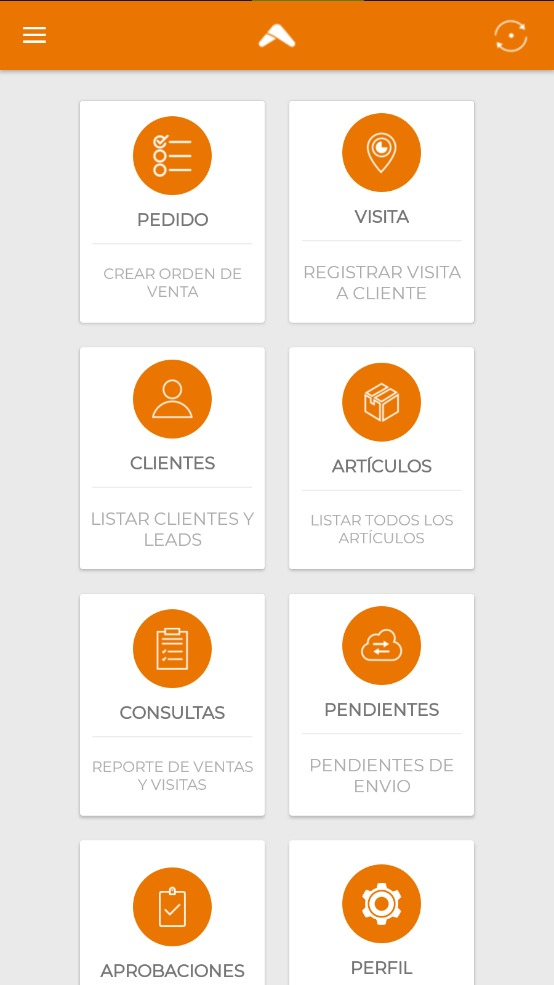
\includegraphics[width=0.2\linewidth,frame=0.5pt 5pt]{img/FV}
            \end{figure}
              \section{Módulo pedido}
              Esté módulo genera ordenes de ventas, en dónde se pueden adjuntar imágenes y consultar stocks en linea por almacen seleccionado.
              \begin{itemize}
              	
              	\item Si hay conexión la orden de venta se envía automáticamente de lo contrario se queda en cola para ser enviada posteriormente.
            \end{itemize}
        Observaciones:
        \begin{itemize}
        	\item  Optimizar el manejo del Transporte.
        	\item  se hacen detracciones? cuando superan los S/400.00.
        	\item  Se maneja como un item adicional o como detalle de la factura? Actualmente la empresa lo tiene como un Item.
        	\item  Se maneja como item por que necesitan generar en una factura adicional.
        	\item Conclusión: Transporte Se manejara como un producto adicional en Factura y OV.
        \end{itemize}
             \section{Módulo Visita}
             Esté módulo registra las visitas hechas a los clientes. Si hay conexión la visita se envía automáticamente de lo contrario se queda en cola para ser enviada posteriormente.
             
             \section{Módulo Clientes} 
             En este módulo se visualiza el listado de clientes que se tienen descargados en la aplicación.\\
             Observaciones:
             \begin{itemize}
             	\item Este Modulo deberá contar con la opción  registro de nuevos cliente con las validaciones mínimas para Facturación Electrónica.
             	\item Debera poder registrar clientes como persona natural(DNI) y persona jurídica(RUC 10, 20).
             	\item Debe tener comunicación con Sunat y Reniec para validar a clientes nuevos.
             \end{itemize}
             
             \section{Módulo Artículos}
             En este módulo se visualiza el listado de artículos que se tiene descargados en la aplicación, y se puede ver el detalle de:
             \begin{itemize}
             	\item Stock por almacén
             	\item Lista de precios
             \end{itemize}
             
             \section{Módulo Consultas}
             En este módulo se hacen consultas en línea de Órdenes de Venta, Facturas y Visitas
             
             \section{Módulo Pendientes}
             En este módulo se podrá ver la cola de pendientes de Órdenes de Venta y Visitas. Dónde se podrá enviar masiva-mente o eliminar elementos de la cola.
             
             \section{Módulo Aprobaciones}
             En este módulo se visualizan las órdenes de venta que pasan por flujo de aprobación y se decide si estas se aprueban o desaprueban.
             \section{Comprobantes y pagos}
                Se generan automáticamente si esta disponible la conexión; de lo contrario se quedan en cola esperando la conexión para emitir los documentos de forma agrupada.
             \chapter{Observaciones}
             \begin{itemize}
             	\item *** Manejar precios especiales de socio de negocio y descuentos por cantidad y periodo.
             	\item *** No se ha definido una lista de precios.
             	\item *** Lista de precios podría incluir IGV en el precio unitario de venta.
             	\item *** Las Horas estimadas serán actualizadas después de levantar estas observaciones.
             \end{itemize}
             \chapter{Horas de Desarrollo}
             \section{Punto de Ventas}
             \begin{table}[htbp]
             	\small
             	\centering
             	
             	\begin{tabular}{llr}       		
             		\# & Actividad & HORAS HOMBRE\\
             		\midrule
             		1 &	CONFIGURACION INICIAL	& 12 \\
             		2 &	MODULOS ADICIONALES POS	& 0 \\
             		3 &	REQUERIMIENTOS ADICIONALES DEL CLIENTE	& 0 \\
             		4 &	CONSUMO ADICIONAL SERVICIOS SAP	& 0 \\
             		5 &	SERVICE LAYER DESARROLLO XS	& 0 \\
             		6 &	DESARROLLO SERVICE SECURITY	& 0 \\
             		7 &	CONTROL DE CALIDAD	& 0 \\
             		\bottomrule
             		Total & &12 \\
             	\end{tabular}%
             \end{table}%
             \section{Fuerza de Ventas}
             \begin{table}[htbp]
             	\small
             	\centering
             	
             	\begin{tabular}{llr}       		
             		\# & Actividad & HORAS HOMBRE\\
             		\midrule
             		1 &	CONFIGURACIÓN INICIAL	& 12 \\
             		2 &	MÓDULOS ADICIONALES POS	& 0 \\
             		3 &	REQUERIMIENTOS ADICIONALES DEL CLIENTE	& 0 \\
             		4 &	CONSUMO ADICIONAL SERVICIOS SAP	& 0 \\
             		5 &	SERVICE LAYER DESARROLLO XS	& 0 \\
             		6 &	DESARROLLO SERVICE SECURITY	& 0 \\
             		7 &	CONTROL DE CALIDAD	& 0 \\
             		\bottomrule
             		Total & & 12 \\
             	\end{tabular}%
             \end{table}%
    \end{sloppypar}
\end{document}
